\scanpage{26}
1) groupe alg. $\boxed{G}$ sur $\mathbf Q_p$.
(Il dépend en fait du choix de $\Omega$. cf plus bas 2°)

2) Hom
\[
\boxed{\rho:\pi\longrightarrow G(\mathbf Q_p)}
\]
[L'op. de $\pi=\operatorname{Aut}_L(\Omega)$ sur $G=G^{(\Omega)}$ est donnée par
$\sigma\longmapsto\mathrm{int}(\rho(\sigma))$

\deleted{3)} On fait opérer $\pi$ sur $G_\Omega$ \uline{diagonalement}, soit $G_\Omega^!$.

3) Hom
\[
\boxed{j^!_{\unsure{\Omega}}:G_{m\Omega}\longrightarrow G_\Omega^!}
\]
\margin{inv. par $\pi$}
\margin{$G_\Omega^{\unsure{!|1}}$}

On appelle \deleted{$\unsure{S_\Omega(1)|S(1)}$}\inserted{$S_\Omega$}
\deleted{$\unsure{T_\Omega}$} le \deleted{$\unsure{T}$}
$\Omega$-module inversible $T_p(\Omega)^{\unsure{*|\#}}\otimes_{\mathbf Z_p}\Omega$
avec op. diagonale de $\pi$, \deleted{\illegible{1}} et $\tau_\Omega$ le $G_{m\Omega}$ torseur associé.
Posons
\deleted{\[
\tau\wedge_{\unsure{G_{m\Omega}}}\Phi
\unsure{\wedge}_{G_{m\Omega}}\unsure{G_\Omega^!}\quad
\unsure{Q_\Omega}\ \unsure{=\tau}\wedge_{\unsure{G_{m\Omega}}}\unsure{G_\Omega^!}
\]}
\inserted{\figure{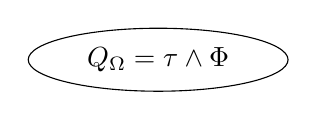
\begin{tikzpicture}
\node at (1.6,0) {$Q_\Omega=\tau\wedge\Phi$};
\draw (1.6,0) ellipse (1.65 and 0.4);
\end{tikzpicture}}}
torseur \inserted{à dr} sur $G_\Omega$
\[
\text{d'où}\quad \uline{G_\Omega^!\text{ tordu}}\text{ par }(\tau,j),
\quad\text{soit }\figure{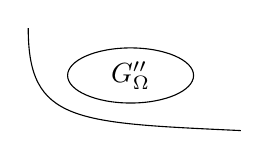
\begin{tikzpicture}[baseline=0pt]
\node at (0.8,0.3) {$G''_\Omega$};
\draw (0.8,0.3) ellipse (0.8 and 0.35);
\draw (-0.5,0.9) .. controls (-0.5,-0.3) and (0.1,-0.3) .. (2.2,-0.4);
\end{tikzpicture}}
\]
[Correspond au foncteur fibré \inserted{(gradué)} sur $\operatorname{Rep}(G)$
\diagram{\begin{tikzcd}
G_{m\Omega}\arrow[r,"j_\Omega^{\unsure{*|\#}}"]&G''_\Omega
\end{tikzcd}}
\[
M\longrightarrow\sum\operatorname{gr}_j^i(M)_\Omega\otimes S_\Omega(-i)
=\operatorname{Hdg}_\Omega(M)
\]

\margin{$\unsure{\angle|4}$}
\uline{Axiome} Le \deleted{foncteur}\inserted{$(T_{\mathrm{Hdg}})$}
$Q_\Omega$ \deleted{\unsure{sur}} se descend à $L$
en un $G_L$-torseur $Q_L$
\figure{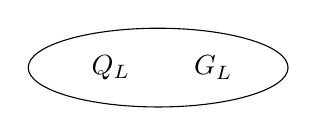
\begin{tikzpicture}
\node at (0.7,0) {$Q_L$};\node at (2,0) {$G_L$};
\draw (1.3,0) ellipse (1.65 and 0.5);
\end{tikzpicture}}
(unique à isom unique près)
en un $G''_L$, et
\diagram{\begin{tikzcd}
G_{mL}\arrow[r,"j_L"]&G''_L
\end{tikzcd}}
Correspond : fct fibré gradué $\operatorname{Hdg}_L$

\margin{\uline{NB} Un $j$ satisfaisant aux conditions est \unsure{unique}.
Signifie que les $\unsure{M_\Omega^!|M_\Omega}$ sont \uline{de Hodge}.
Du moins si}

\figure{\begin{tikzpicture}[x=1cm,y=1cm]
\draw (0,0) .. controls (2,0.4) and (4,-0.2) .. (8,0.1);
\end{tikzpicture}}
\margin{$\unsure{Q|\alpha}$}
Il y a deux foncteurs fibres de $\operatorname{Rep}(G)$ dans $\operatorname{Mod}(\Omega,\pi)$
\[
\begin{array}{ll}
a)\quad M\longrightarrow M_\Omega &
\text{\unsure{opérations|opération} provenant des op. \unsure{canoniques} de }\pi\text{ sur }\Omega\\
b)\quad M\mathrel{-}M_\Omega^! &\text{opération diagonale}
\end{array}
\]
-- foncteurs $T_{p\Omega}$ et $T^!_{p\Omega}$

\deleted{Après oubli des op.} On a là un \deleted{$(\Omega,\pi)$} torseur \inserted{à droite} sur
$(\Omega,\pi)$ de groupe $G_\Omega$, soit $\Phi_\Omega$, donné par le 1-cocycle
\[
\rho:\pi\mathrel{-}G(\mathbf Q_p)\subset H^0(\Omega,\unsure{\deleted{\pi}|\pi};G_\Omega)=G(\unsure{L|\Omega}).
\]
Le \deleted{groupe} $\uline{\operatorname{Aut}}_{G_{\Omega,\pi}}(\Phi)$ est $G_\Omega^!$.
\margin{$(\Omega,\pi)$}
\figure{\begin{tikzpicture}
\draw (0,0) .. controls (0.6,0.1) and (1.5,-0.1) .. (1.7,0.45);
\end{tikzpicture}}
\margin{25}
